% Provenance (never printed): see sources/outline_sources.md (Year 1: the wind-driven
% circulation, gyres, Ekman transport and upwelling, western boundary currents, the
% meridional overturning circulation and the water masses). Exercise and problem values in
% the Book 3 scratch calculator calc/ch29.py; figures from figdata/bachelor-1/
% ekman_hodograph.py (Ekman's solution with Ekman's constants) and stommel_gyre.py
% (Stommel's 1948 model, exercise parameters), the world map from figdata/shared/geo.py.
% Physics owns the Coriolis force (recalled). Book 1 (g8) gave the surface currents and
% the gyres in words, Book 2 (g10) upwelling: re-founded here with the Ekman balance.
% Ch. 26 owns the T-S diagram and the water masses, ch. 28 the Coriolis parameter, the
% geostrophic wind and the mean meridional streamfunction. The Sverdrup balance, the
% vorticity argument and the derivation of the Ekman spiral are the Year 3 volume's; ENSO
% the Year 2 volume's.
\chapter{De circulatie van de oceaan}\label{ch:b1:ocean-circulation}

In 1992, tijdens een storm in de Noord-Pacifische Oceaan, viel een container van een schip dat van Hongkong naar de Verenigde Staten voer over boord. Hij brak open en liet ongeveer \num{29000} rubberen eendjes en ander badspeelgoed los, dat wegdreef en ver en wijd reisde; de plaatsen waar sommige later werden gevonden, hielpen wetenschappers de stromingen te begrijpen die hen hadden meegevoerd. Drijvend speelgoed volgt het oppervlaktewater, en het oppervlaktewater van de oceanen dwaalt niet willekeurig rond: het draait in bekkenbrede \omterm{def:b1:ocean-circulation:gyre}{gyres}, stroomt in smalle stromen noordwaarts langs de westkusten van de oceanen, en stijgt of daalt op enkele uitgekozen plaatsen. Dit hoofdstuk legt uit hoe de wind het bovenste deel van de oceaan in beweging zet, waarom het water loopt onder rechte hoeken op de wind die het duwt, waarom de sterkste stromingen de westzijden van de oceanen volgen, en hoe een langzame omwenteling water naar de diepte brengt en weer terug.
% ledger: noaa:floatees

\begin{omfigure}
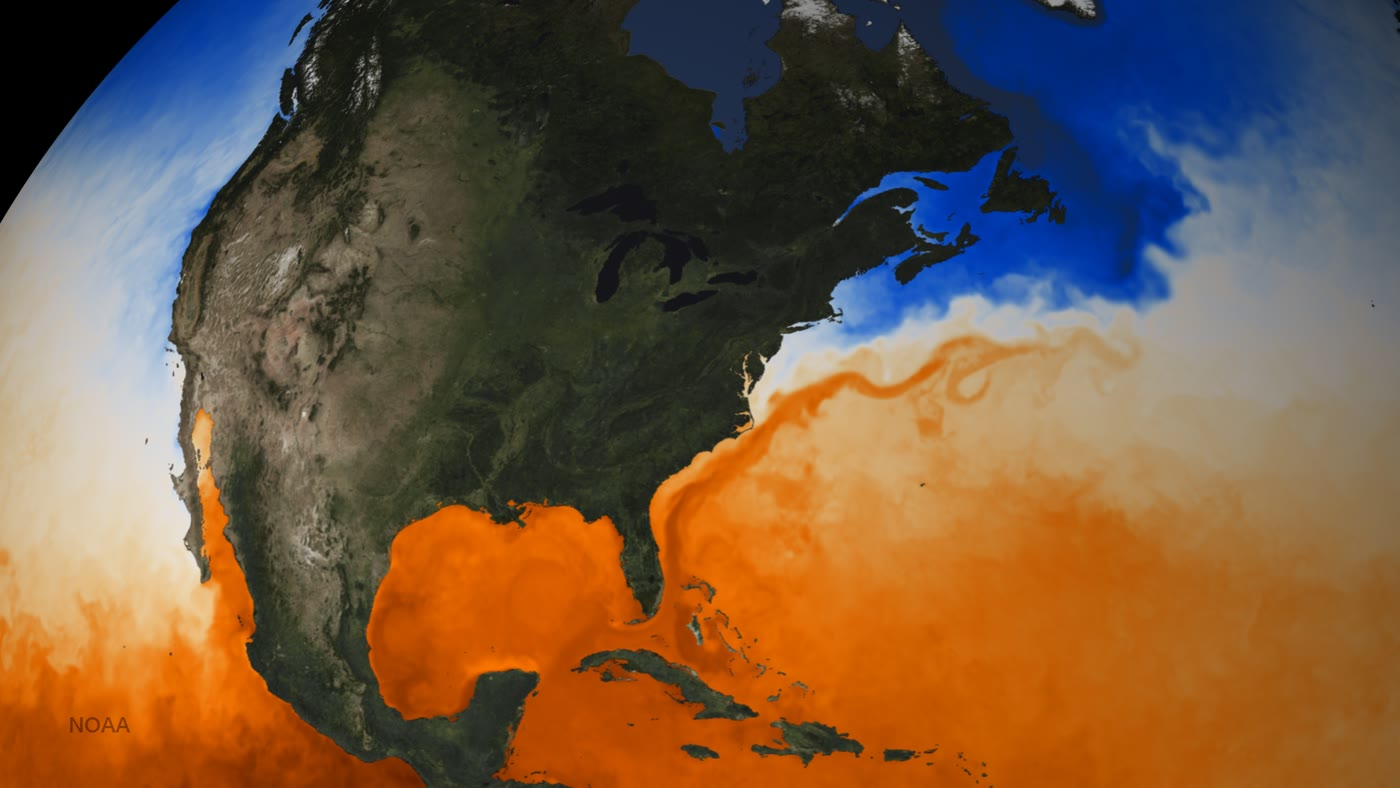
\includegraphics[width=0.85\linewidth]{images/book3/b1-gulf-stream-sst.jpg}

{\small De temperatuur van het zeeoppervlak rond Noord-Amerika begin juni 2016, uit satellietgegevens (warm water in oranje, koud water in blauw). De Golfstroom verlaat de kust van de Verenigde Staten als een warm, meanderend lint en steekt de Atlantische Oceaan over naar Europa; op dezelfde breedtegraden is het water voor de Pacifische kust veel koeler dan voor de Atlantische kust. (NOAA, NESDIS, publiek domein, via Wikimedia Commons.)}
\label{fig:b1:ocean-circulation:sst}
\end{omfigure}
% ledger: commons:gulf-stream-sst, noaa:gulf-stream-heat

\begin{recall}
De natuurkundedelen geven de Coriolis-kracht. \Cref{ch:b1:atmospheric-circulation} schreef haar horizontale deel als $-f\,\vec k\times\vec v$, met de \omterm{def:b1:atmospheric-circulation:coriolis-parameter}{Coriolisparameter}
$f = 2\Omega\sin\varphi$ ($\Omega = \qty{7.292e-5}{rad.s^{-1}}$), en vond de \omterm{def:b1:atmospheric-circulation:winds}{passaten}, oostenwinden tussen de evenaar en ongeveer \ang{30}, en de \omterm{def:b1:atmospheric-circulation:winds}{westenwinden} daarachter; het definieerde ook de \omterm{def:b1:atmospheric-circulation:streamfunction}{gemiddelde meridionale stroomfunctie} van een omwenteling. \Cref{ch:b1:fluid-envelopes-structure} gaf de \omterm{def:b1:fluid-envelopes-structure:ocean-layers}{gemengde laag} en de thermocline, de dichtheid van zeewater, het \omterm{def:b1:fluid-envelopes-structure:ts-diagram}{T--S-diagram} en de \omterm{def:b1:fluid-envelopes-structure:ts-diagram}{watermassa}'s van de Zuidelijke Atlantische Oceaan, en \cref{ch:b1:radiation-heat-transport} het poolwaartse warmtetransport dat door atmosfeer en oceaan wordt gedeeld. Boek~1 beschreef de oppervlaktestromingen en de grote \omterm{def:b1:ocean-circulation:gyre}{gyres}; Boek~2 de \omterm{def:b1:ocean-circulation:upwelling}{opwelling} van koud water langs sommige kusten.
% ledger: earth:Trot, nos:gyres
\end{recall}

\section{De wind en de oppervlaktestromingen}\label{sec:b1:ocean-circulation:wind}

De wind beweegt de zee door er over te schuren. Zijn kracht is over het oppervlak verdeeld en wordt, net als een druk, per oppervlakte-eenheid gemeten.

\begin{definition}[Windschuifspanning]\label{def:b1:ocean-circulation:wind-stress}
De \emph{windschuifspanning}\index{windschuifspanning} $\vec T$ is de horizontale kracht per oppervlakte-eenheid die de wind op het zeeoppervlak uitoefent, in pascal. Zij is de neerwaartse overdracht van de horizontale impuls van de lucht naar de oceaan, en wijst bijna in de richting van de wind. Haar grootte wordt gegeven door de bulkformule
\[
  T = \rho_a C_D U_{10}^2,
\]
waarin $\rho_a = \qty{1.3}{kg.m^{-3}}$ de dichtheid van lucht is, $U_{10}$ de windsnelheid op \qty{10}{m} boven de zee en $C_D$ een dimensionloze weerstandscoëfficiënt.
\end{definition}
% ledger: stewart:wind-stress

De weerstandscoëfficiënt wordt gemeten met snelle instrumenten die de turbulente schommelingen van de wind enkele meters boven de golven registreren. Voor neutraal stabiele lucht geven de metingen van Yelland en Taylor
\[
  1000\,C_D = 0.29 + \frac{3.1}{U_{10}} + \frac{7.7}{U_{10}^2}
  \quad (\qtyrange{3}{6}{m/s}),
  \qquad
  1000\,C_D = 0.60 + 0.071\,U_{10}
  \quad (\qtyrange{6}{26}{m/s}),
\]
met $U_{10}$ in meter per seconde. Een wind van \qty{10}{m/s} heeft $C_D =
\num{1.31e-3}$ en oefent $T = 1.3 \times \num{1.31e-3} \times 100 =
\qty{0.170}{Pa}$; een wind van \qty{5}{m/s}, \qty{0.040}{Pa}; een storm van
\qty{20}{m/s}, \qty{1.05}{Pa}. Verdubbeling van de wind van 10 tot \qty{20}{m/s}
vermenigvuldigt de schuifspanning met $6.2$, niet met $4$: ruwere zeeën grijpen de wind harder aan. Deze spanningen zijn heel klein, een miljoenste van de luchtdruk, maar zij werken zonder onderbreking op de hele oceaan.
% ledger: stewart:drag-coefficient (computed in figdata/bachelor-1/ekman_hodograph.py and calc/ch29.py)

Het patroon van de spanning volgt dat van de winden. Tussen de \omterm{def:b1:atmospheric-circulation:winds}{passaten} van de tropen, die naar het westen waaien, en de \omterm{def:b1:atmospheric-circulation:winds}{westenwinden} van de middelbreedten, die naar het oosten waaien, wordt het oppervlaktewater van elk oceaanbekken in draaiing gebracht.

\begin{definition}[Gyre; subtropische en subpolaire gyres]\label{def:b1:ocean-circulation:gyre}
Een \emph{gyre}\index{gyre} is een groot systeem van ronddraaiende oceaanstromingen dat een oceaanbekken vult. Een \emph{subtropische gyre}\index{subtropische gyre} ligt tussen de \omterm{def:b1:atmospheric-circulation:winds}{passaten} en de \omterm{def:b1:atmospheric-circulation:winds}{westenwinden} en draait rechtsom op het noordelijk halfrond en linksom op het zuidelijk. Een \emph{subpolaire gyre}\index{subpolaire gyre} ligt aan de poolwaartse kant van de \omterm{def:b1:atmospheric-circulation:winds}{westenwinden} en draait de andere kant op.
\end{definition}
% ledger: nos:gyre-def, nos:boundary-currents, stewart:north-atlantic

Er zijn vijf \omterm{def:b1:ocean-circulation:gyre}{subtropische gyres}, in de Noord- en Zuid-Atlantische Oceaan, de Noord- en Zuid-Pacifische Oceaan en de Indische Oceaan; geen ervan overspant de evenaar. In de Noord-Atlantische Oceaan wordt de \omterm{def:b1:ocean-circulation:gyre}{subtropische gyre} in het westen gesloten door de Golfstroom langs de kust van de Verenigde Staten en in het oosten door de Canarische stroom voor Afrika; noordelijk daarvan draait de \omterm{def:b1:ocean-circulation:gyre}{subpolaire gyre} linksom, met de Noord-Atlantische stroom aan haar zuidzijde en de Labradorstroom die langs haar westzijde naar het zuiden stroomt. Op lage breedtegraden zijn de westwaarts gerichte equatoriale stromingen van de Atlantische en de Stille Oceaan gescheiden door een oostwaartse tegenstroom. De \omterm{def:b1:ocean-circulation:gyre}{gyres} zijn niet symmetrisch: elke \omterm{def:b1:ocean-circulation:gyre}{subtropische gyre} wordt aan de westzijde van haar bekken gesloten door een sterke, smalle stroom en aan de oostzijde door een zwakke, brede stroom. Rond Antarctica, waar geen continent het tegenhoudt, stroomt de Antarctische Circumpolaire Stroom oostwaarts om de aarde, aangedreven door de \omterm{def:b1:atmospheric-circulation:winds}{westenwinden} van de Zuidelijke Oceaan.
% ledger: nos:boundary-currents, stewart:north-atlantic, stewart:heat-conveyor, lien:kuroshio, donohue:acc, stewart:acc

\begin{omfigure}
\begin{tikzpicture}
\begin{axis}[ommap, width=0.98\linewidth, xtick={-180,-120,...,180}, ytick={-60,-30,0,30,60}]
% land: figdata/shared/geo.py; ledger: data:ne-land. Arrows placed by hand from the
% ledgered pattern: nos:boundary-currents, stewart:north-atlantic, lien:kuroshio,
% donohue:acc, stewart:acc
\addplot[fill=omLithAlluv, draw=black!45, line width=0.2pt, forget plot] table {figdata/out/shared-geo-land.dat};
% North Atlantic subtropical gyre (clockwise)
\addplot[omThm, line width=1.1pt, -{Stealth[length=4pt]}, smooth] coordinates {(-80,26) (-77,32) (-70,37) (-58,40) (-44,41)};
\addplot[omThm, line width=1.1pt, -{Stealth[length=4pt]}, smooth] coordinates {(-38,40) (-28,39) (-20,36)};
\addplot[omThm, line width=1.1pt, -{Stealth[length=4pt]}, smooth] coordinates {(-19,32) (-21,24) (-26,17)};
\addplot[omThm, line width=1.1pt, -{Stealth[length=4pt]}, smooth] coordinates {(-32,14) (-45,13) (-60,15)};
% North Atlantic subpolar gyre (anticlockwise)
\addplot[omDef, line width=1.1pt, -{Stealth[length=4pt]}, smooth] coordinates {(-40,47) (-28,52) (-18,57)};
\addplot[omDef, line width=1.1pt, -{Stealth[length=4pt]}, smooth] coordinates {(-24,61) (-35,62) (-44,59)};
\addplot[omDef, line width=1.1pt, -{Stealth[length=4pt]}, smooth] coordinates {(-55,59) (-56,53) (-51,47)};
% North Pacific subtropical gyre (clockwise)
\addplot[omThm, line width=1.1pt, -{Stealth[length=4pt]}, smooth] coordinates {(123,19) (125,26) (133,32) (143,36) (156,38)};
\addplot[omThm, line width=1.1pt, smooth] coordinates {(162,39) (172,40) (180,40.5)};
\addplot[omThm, line width=1.1pt, -{Stealth[length=4pt]}, smooth] coordinates {(-180,40.5) (-165,41) (-148,40)};
\addplot[omThm, line width=1.1pt, -{Stealth[length=4pt]}, smooth] coordinates {(-133,37) (-128,29) (-122,20)};
\addplot[omThm, line width=1.1pt, -{Stealth[length=4pt]}, smooth] coordinates {(-125,13) (-150,12) (-175,13)};
\addplot[omThm, line width=1.1pt, -{Stealth[length=4pt]}, smooth] coordinates {(170,13) (152,14) (135,15)};
% South Atlantic subtropical gyre (anticlockwise)
\addplot[omThm, line width=1.1pt, -{Stealth[length=4pt]}, smooth] coordinates {(2,-8) (-15,-9) (-30,-9)};
\addplot[omThm, line width=1.1pt, -{Stealth[length=4pt]}, smooth] coordinates {(-34,-14) (-39,-24) (-47,-34)};
\addplot[omThm, line width=1.1pt, -{Stealth[length=4pt]}, smooth] coordinates {(-42,-40) (-20,-40) (2,-38)};
\addplot[omThm, line width=1.1pt, -{Stealth[length=4pt]}, smooth] coordinates {(10,-31) (9,-23) (6,-15)};
% South Pacific subtropical gyre (anticlockwise)
\addplot[omThm, line width=1.1pt, -{Stealth[length=4pt]}, smooth] coordinates {(-88,-10) (-120,-11) (-160,-12)};
\addplot[omThm, line width=1.1pt, -{Stealth[length=4pt]}, smooth] coordinates {(160,-16) (157,-26) (162,-35)};
\addplot[omThm, line width=1.1pt, -{Stealth[length=4pt]}, smooth] coordinates {(-170,-40) (-140,-41) (-105,-39)};
\addplot[omThm, line width=1.1pt, -{Stealth[length=4pt]}, smooth] coordinates {(-82,-36) (-82,-27) (-85,-17)};
% Indian Ocean subtropical gyre (anticlockwise)
\addplot[omThm, line width=1.1pt, -{Stealth[length=4pt]}, smooth] coordinates {(98,-13) (80,-14) (60,-15)};
\addplot[omThm, line width=1.1pt, -{Stealth[length=4pt]}, smooth] coordinates {(47,-22) (40,-29) (33,-34)};
\addplot[omThm, line width=1.1pt, -{Stealth[length=4pt]}, smooth] coordinates {(50,-38) (75,-37) (100,-35)};
\addplot[omThm, line width=1.1pt, -{Stealth[length=4pt]}, smooth] coordinates {(108,-31) (106,-24) (102,-18)};
% Antarctic Circumpolar Current (eastward)
\addplot[omMeth, line width=1.4pt, -{Stealth[length=5pt]}, smooth] coordinates {(-62,-58) (-40,-55) (-15,-52)};
\addplot[omMeth, line width=1.4pt, -{Stealth[length=5pt]}, smooth] coordinates {(5,-52) (40,-50) (75,-50)};
\addplot[omMeth, line width=1.4pt, -{Stealth[length=5pt]}, smooth] coordinates {(95,-51) (130,-53) (165,-56)};
\addplot[omMeth, line width=1.4pt, -{Stealth[length=5pt]}, smooth] coordinates {(-170,-58) (-130,-59) (-85,-59)};
\node[font=\scriptsize, anchor=west, fill=white, fill opacity=0.8, text opacity=1, inner sep=1pt] at (axis cs:-66,31) {Golfstroom};
\node[font=\scriptsize, anchor=west, fill=white, fill opacity=0.8, text opacity=1, inner sep=1pt] at (axis cs:-11,25) {Canarische};
\node[font=\scriptsize, anchor=east, fill=white, fill opacity=0.8, text opacity=1, inner sep=1pt] at (axis cs:-58,52) {Labrador};
\node[font=\scriptsize, anchor=west, fill=white, fill opacity=0.8, text opacity=1, inner sep=1pt] at (axis cs:142,28) {Kuroshio};
\node[font=\scriptsize, anchor=north, fill=white, fill opacity=0.8, text opacity=1, inner sep=1pt] at (axis cs:-150,9) {Noord-equatoriale};
\node[font=\scriptsize, anchor=north, fill=white, fill opacity=0.8, text opacity=1, inner sep=1pt] at (axis cs:0,-62) {Antarctische Circumpolaire Stroom};
\end{axis}
\end{tikzpicture}

{\small De \omterm{def:b1:ocean-circulation:gyre}{gyres} van het oppervlak van de oceaan (schematische pijlen op een kaart van de landmassa's).
Donkerrood: de vijf \omterm{def:b1:ocean-circulation:gyre}{subtropische gyres}, rechtsom op het noordelijk halfrond en linksom op het zuidelijk, elk met een smalle \omterm{def:b1:ocean-circulation:wbc}{westelijke randstroom}; blauw: de \omterm{def:b1:ocean-circulation:gyre}{subpolaire gyre} van de Noord-Atlantische Oceaan; groen: de Antarctische Circumpolaire Stroom. Genoemd zijn alleen de stromingen die in de tekst worden besproken. De pijlen tonen de richting van de stroming, niet haar snelheid.}
\label{fig:b1:ocean-circulation:gyres}
\end{omfigure}
% ledger: data:ne-land, nos:boundary-currents, stewart:north-atlantic, lien:kuroshio, donohue:acc

Twee kenmerken van dit patroon vragen om uitleg. Het eerste is de draairichting: de \omterm{def:b1:atmospheric-circulation:winds}{passaten} waaien naar het westen aan de evenaarszijde van een \omterm{def:b1:ocean-circulation:gyre}{subtropische gyre}, maar de stromingen van de \omterm{def:b1:ocean-circulation:gyre}{gyre} volgen de winden niet eenvoudig, en het oppervlaktewater drijft er onder een hoek van af. Het tweede is de asymmetrie: de terugstroom van een \omterm{def:b1:ocean-circulation:gyre}{gyre} wordt tegen de westzijde van haar bekken samengedrukt. Beide komen voort uit de rotatie van de aarde.

\section{Ekmantransport}\label{sec:b1:ocean-circulation:ekman}

\begin{history}[Nansen en Ekman, 1898--1905]
Tijdens zijn expeditie in het Noordpoolgebied merkte Fridtjof Nansen op dat de wind het zee-ijs niet langs de wind dreef, maar onder een hoek van \ang{20} tot \ang{40} naar rechts, kijkend met de wind mee. Hij redeneerde dat drie krachten op het bewegende ijs in evenwicht moesten zijn: de duw van de wind, de wrijving van het water en de Coriolis-kracht. Hij vroeg de meteoroloog Vilhelm Bjerknes om een van zijn studenten de invloed van de rotatie van de aarde op door wind gedreven stromingen te laten onderzoeken. De student, Walfrid Ekman, werkte de theorie uit voor zijn proefschrift in Uppsala en breidde haar in 1905 uit. Zijn oplossing is nog steeds het startpunt van de theorie van de door wind gedreven oceaan.
\end{history}
% ledger: stewart:ekman-layer, nos:ekman-spiral

\begin{definition}[Ekmanlaag, Ekmantransport, Ekmanspiraal]\label{def:b1:ocean-circulation:ekman}
De \emph{Ekmanlaag}\index{Ekmanlaag} is de dunne oppervlaktelaag van de oceaan, hooguit enkele honderden meters dik, waarin de spanning van de wind door turbulente wrijving naar beneden wordt overgedragen en door de Coriolis-kracht in evenwicht wordt gehouden. Het \emph{Ekmantransport}\index{Ekmantransport} is de massa water die de laag per seconde meeneemt over een verticale strook van \qty{1}{m} breed, van het oppervlak tot onder de laag:
\[
  \vec M = \int_{-d}^{0} \rho\,\vec v\,\mathrm dz \quad (\unit{kg.m^{-1}.s^{-1}});
\]
gedeeld door de dichtheid is het een volumetransport per meter, in
\unit{m^2.s^{-1}}. De \emph{Ekmanspiraal}\index{Ekmanspiraal} is de draaiing en verzwakking van de stroming met de diepte in de laag. Transporten van de oceaan worden uitgedrukt in \emph{sverdrups}\index{sverdrup (unit)}: \qty{1}{\sverdrup} $=
\qty{e6}{m^3.s^{-1}}$.
\end{definition}
% ledger: stewart:ekman-layer, stewart:ekman-transport

\begin{theorem}[Ekmantransport]\label{thm:b1:ocean-circulation:ekman}
In een stationaire toestand, ver van de kusten, boven water dat veel dieper is dan de \omterm{def:b1:ocean-circulation:ekman}{Ekmanlaag}, hangt het \omterm{def:b1:ocean-circulation:ekman}{Ekmantransport} alleen af van de \omterm{def:b1:ocean-circulation:wind-stress}{windschuifspanning} $\vec T$ en van de \omterm{def:b1:atmospheric-circulation:coriolis-parameter}{Coriolisparameter} $f$:
\[
  \vec M = \frac{1}{f}\,\vec T\times\vec k,
  \qquad |\vec M| = \frac{|\vec T|}{|f|}.
\]
Het staat loodrecht op de \omterm{def:b1:ocean-circulation:wind-stress}{windschuifspanning}, rechts ervan op het noordelijk halfrond en links ervan op het zuidelijk.
\end{theorem}
% ledger: stewart:ekman-transport

\begin{proof}
Laat $\vec\tau(z)$ de horizontale spanning zijn die het water boven het niveau $z$
uitoefent op het water eronder. Aan het oppervlak is zij de \omterm{def:b1:ocean-circulation:wind-stress}{windschuifspanning}, $\vec\tau(0) =
\vec T$; onder de laag, waar de door de wind gedreven stromingen zijn uitgedoofd, verdwijnt zij,
$\vec\tau(-d) = \vec 0$. Een dunne plak tussen $z$ en $z + \mathrm dz$, met een horizontaal oppervlak van één eenheid, ontvangt
$\vec\tau(z + \mathrm dz)$ op haar bovenvlak en
$-\vec\tau(z)$ op haar ondervlak: de netto wrijvingskracht is $(\partial\vec
\tau/\partial z)\,\mathrm dz$. Haar massa is $\rho\,\mathrm dz$, en de horizontale
Coriolis-kracht erop is $-f\,\vec k\times\vec v\,\rho\,\mathrm dz$. In een stationaire
toestand, zonder horizontale verandering van de ene plaats naar de andere, houden de twee elkaar in evenwicht:
\[
  -f\rho\,\vec k\times\vec v + \frac{\partial\vec\tau}{\partial z} = \vec 0 .
\]
Integrerend van $-d$ tot $0$,
\[
  -f\,\vec k\times\vec M + \vec\tau(0) - \vec\tau(-d) = \vec 0,
  \qquad\text{dat is}\qquad \vec k\times\vec M = \frac{\vec T}{f}.
\]
Voor een horizontale vector geldt $\vec k\times(\vec k\times\vec M) = -\vec M$; door
$\vec k\times$ van beide zijden te nemen volgt $-\vec M = \vec k\times\vec T/f$, dus $\vec M =
\vec T\times\vec k/f$. De vector $\vec T\times\vec k$ is $\vec T$ over \ang{90} gedraaid
met de klok mee, gezien van boven: naar rechts van de wind als $f > 0$, naar links als $f < 0$.
Haar grootte is $|\vec T|$.
\end{proof}

Het resultaat hangt niet af van hoe de wrijving binnen de laag werkt, wat slecht bekend is: alleen de spanning aan de top en haar verdwijnen aan de onderkant gaan erin.
Dit maakt het transport veel robuuster dan de snelheden zelf. Het water van de hele laag, samen genomen, beweegt loodrecht op de wind, een resultaat dat vreemd lijkt totdat men bedenkt dat de Coriolis-kracht over een dag of langer de tijd heeft om elke stroming te draaien.

\begin{example}[Het transport onder een frisse bries]\label{ex:b1:ocean-circulation:transport}
Een wind van \qty{10}{m/s} die naar het noorden waait op \ang{35} N oefent
$T = \qty{0.170}{Pa}$ uit. Met $f = 2\Omega\sin\ang{35} = \qty{8.365e-5}{s^{-1}}$, is het
\omterm{def:b1:ocean-circulation:ekman}{Ekmantransport} $0.170/(\num{8.365e-5}) = \qty{2036}{kg.m^{-1}.s^{-1}}$, naar het oosten. Met $\rho = \qty{1027}{kg.m^{-3}}$ is dit \qty{1.98}{m^3.s^{-1}} per
elke meter gemeten dwars op het transport: over een lijn van \qty{1000}{km} lang, ongeveer
\qty{2}{\sverdrup}.
\end{example}
% ledger: stewart:drag-coefficient, stewart:ekman-constants, earth:Trot (computed in calc/ch29.py)

De stelling is op zee getoetst. Over \ang{11} N in de Atlantische Oceaan, waar de \omterm{def:b1:atmospheric-circulation:winds}{passaten} naar het westen waaien, is het \omterm{def:b1:ocean-circulation:ekman}{Ekmantransport} naar het noorden gericht; rechtstreeks gemeten met een stroomprofiler kwam het uit op
\qty[uncertainty-mode=separate]{12.0 \pm 5.5}{\sverdrup}, tegen
\qty[uncertainty-mode=separate]{8.8 \pm 1.9}{\sverdrup} berekend uit de winden die tijdens de meetvaart zijn gemeten, en
\qty[uncertainty-mode=separate]{13.5 \pm 0.3}{\sverdrup} uit winden die over vele jaren zijn gemiddeld.
% ledger: stewart:ekman-transport

Hoe de stroming met de diepte in de laag verdeeld is, hangt van de wrijving af. Ekman koos het eenvoudigste model, een turbulente wrijving evenredig met de verticale afschuiving van de stroming,
$\vec\tau = \rho A_z\,\partial\vec v/\partial z$, met
een constante wervelviscositeit $A_z$.

\begin{proposition}[De Ekmanspiraal]\label{prop:b1:ocean-circulation:spiral}
Voor een stationaire \omterm{def:b1:ocean-circulation:wind-stress}{windschuifspanning} $T$ naar het noorden boven een diepe, homogene oceaan in het
noordelijk halfrond, met een constante wervelviscositeit $A_z$, is de stroming op hoogte $z
\leq 0$ gelijk aan
\[
  u = V_0\,e^{az}\cos\Bigl(\frac\pi4 + az\Bigr),\qquad
  v = V_0\,e^{az}\sin\Bigl(\frac\pi4 + az\Bigr),\qquad
  a = \sqrt{\frac{f}{2A_z}},\quad V_0 = \frac{T}{\rho\sqrt{fA_z}},
\]
met $u$ oostwaarts en $v$ noordwaarts. Aan het oppervlak stroomt de stroming onder \ang{45} naar rechts van de wind; met de diepte verzwakt zij als $e^{az}$ en draait zij verder naar rechts. Op de diepte $D_E = \pi/a$, de Ekmandiepte, stroomt zij tegen de oppervlaktestroom in
met $e^{-\pi} = \num{0.043}$ van haar snelheid.
\end{proposition}
\admitted
% ledger: stewart:ekman-solution

De afleiding lost de twee vergelijkingen $f v + A_z u'' = 0$ en $-f u + A_z v'' =
0$ van het evenwicht uit het bewijs hierboven op; zij wordt gegeven in Boek~5, en
\cref{exo:b1:ocean-circulation:10} controleert dat de formules aan de vergelijkingen voldoen
en dat de spiraal precies het transport van de stelling draagt. Om de spiraal te gebruiken, heeft men $A_z$ nodig, dat niet rechtstreeks wordt gemeten. Ekman verzamelde de
waargenomen snelheden van oppervlaktestromingen en vond, voor $|\varphi| \geq \ang{10}$,
\[
  V_0 = \frac{0.0127\,U_{10}}{\sqrt{\sin|\varphi|}},
  \qquad\text{waaruit volgt}\qquad
  D_E = \frac{7.6\,U_{10}}{\sqrt{\sin|\varphi|}},
\]
in SI-eenheden, met zijn weerstandscoëfficiënt $C_D = \num{2.6e-3}$ en $\rho_a =
\qty{1.25}{kg.m^{-3}}$. Op \ang{35} N onder een wind van \qty{10}{m/s} is $D_E =
\qty{100}{m}$ en $V_0 = \qty{0.17}{m/s}$; de \omterm{def:b1:ocean-circulation:ekman}{Ekmanlaag} varieert van ongeveer
\qty{45}{m} onder zwakke winden op de middelbreedten tot \qty{300}{m} onder een storm in de tropen, en de oppervlaktestroom is \qtyrange{1}{2.5}{\percent} van de wind.
% ledger: stewart:ekman-constants (computed in figdata/bachelor-1/ekman_hodograph.py)

\begin{omfigure}
\begin{tikzpicture}
\begin{axis}[ompt, name=hodo, width=0.5\linewidth, axis equal image, xmin=-6, xmax=22,
  ymin=-6, ymax=17, xlabel={oostwaartse stroming (\unit{cm/s})}, ylabel={noordwaartse stroming (\unit{cm/s})},
  xtick={-5,0,5,10,15,20}, ytick={-5,0,5,10,15}]
% figdata/bachelor-1/ekman_hodograph.py; ledger: stewart:ekman-solution, stewart:ekman-constants
\addplot[black!45, line width=0.6pt] table[x expr=\thisrow{u}*100, y expr=\thisrow{v}*100] {figdata/out/bachelor-1-ekman_hodograph-tips.dat};
\addplot[omDef, line width=0.6pt, -{Stealth[length=3pt]}, quiver={u=\thisrow{u}*100, v=\thisrow{v}*100}]
  table[x expr=0, y expr=0] {figdata/out/bachelor-1-ekman_hodograph-arrows.dat};
\draw[omThm, line width=1.6pt, -{Stealth[length=6pt]}] (axis cs:-3,0) -- (axis cs:-3,14);
\node[font=\scriptsize, text=omThm, anchor=west] at (axis cs:-2.6,13) {wind};
\draw[omMeth, line width=1.6pt, -{Stealth[length=6pt]}] (axis cs:0,-3.2) -- (axis cs:16,-3.2);
\node[font=\scriptsize, text=omMeth, anchor=north] at (axis cs:8,-3.6) {Ekmantransport};
\node[font=\scriptsize, anchor=south west] at (axis cs:11.9,11.9) {oppervlak};
\node[font=\scriptsize, anchor=north east] at (axis cs:-0.3,-0.4) {$D_E$};
\end{axis}
\begin{axis}[ompt, at={(hodo.east)}, anchor=west, xshift=1.4cm, width=0.42\linewidth, height=6.2cm,
  xmin=-4, xmax=14, ymin=-200, ymax=0, xlabel={stroming (\unit{cm/s})}, ylabel={diepte (\unit{m})},
  yticklabel={$\pgfmathprintnumber[fixed]{\tick}$},
  legend style={font=\scriptsize, at={(0.97,0.03)}, anchor=south east, cells={anchor=west}}]
\addplot[black!40, forget plot] coordinates {(0,-200) (0,0)};
\addplot[omDef, line width=1pt] table[x expr=\thisrow{u}*100, y=z] {figdata/out/bachelor-1-ekman_hodograph-profile.dat};
\addlegendentry{oostwaarts}
\addplot[omProp, line width=1pt, dashed] table[x expr=\thisrow{v}*100, y=z] {figdata/out/bachelor-1-ekman_hodograph-profile.dat};
\addlegendentry{noordwaarts}
\addplot[black!50, densely dotted, forget plot] coordinates {(-4,-100.35) (14,-100.35)};
\node[font=\scriptsize, anchor=south east] at (axis cs:13.8,-100.35) {$D_E = \qty{100}{m}$};
\end{axis}
\end{tikzpicture}

{\small Ekmans spiraal onder een wind van \qty{10}{m/s} die naar het noorden waait op \ang{35} N, met de constanten van Ekman. Links: de stroming van boven gezien aan het oppervlak en op elke tiende van de Ekmandiepte $D_E$ tot $D_E$ (blauwe pijlen), de grijze kromme die hun punten verbindt; de oppervlaktestroom is \ang{45} naar rechts van de wind, de diepere zijn zwakker en verder naar rechts gedraaid. Het transport van de hele laag (groen; alleen de richting) staat \ang{90} naar rechts van de wind. Rechts: de twee componenten tegen de diepte.}
\label{fig:b1:ocean-circulation:spiral}
\end{omfigure}
% ledger: stewart:ekman-solution, stewart:ekman-constants

De spiraal is een idealisatie. Metingen van stroommeters op verankerde boeien en van 1503 drijvers die tussen 1987 en 1994 in de Stille Oceaan werden gevolgd, laten zien dat de stroming, gemiddeld over vele dagen, opmerkelijk goed overeenkomt met de theorie van Ekman: de diepte van de laag is bijna de zijne, $7.12\,U_{10}/\sqrt{\sin|\varphi|}$; de oppervlaktestroom is
ongeveer de helft van zijn waarde; de hoek tussen de wind en de oppervlaktestroom is nabij \ang{45} op de middelbreedten; en het transport staat \ang{90} naar rechts van de wind.
Binnen enkele uren wordt het beeld vertroebeld door traagheidsoscillaties, en het evenwicht heeft een wind nodig die een dag of twee gestaag waait om zich te vestigen.
% ledger: stewart:ekman-observed

\section{Opwelling en Ekman-pompen}\label{sec:b1:ocean-circulation:upwelling}

Waar het \omterm{def:b1:ocean-circulation:ekman}{Ekmantransport} niet overal hetzelfde is, hoopt water zich op in sommige plaatsen en wordt het uit andere weggetrokken; het verschil wordt aangevuld door verticale beweging.

\begin{definition}[Opwelling, neerwelling, kustopwelling]\label{def:b1:ocean-circulation:upwelling}
\emph{Opwelling}\index{opwelling} is het opstijgen van water van onderaf in de oppervlaktelaag van de oceaan, om het weggevoerde oppervlaktewater te vervangen; \emph{neerwelling}%
\index{neerwelling} is het zinken van oppervlaktewater waar het zich ophoopt.
\emph{Kustopwelling}\index{kustopwelling} doet zich voor waar een wind die langs een kust waait een \omterm{def:b1:ocean-circulation:ekman}{Ekmantransport} van de kust weg drijft: op het noordelijk halfrond,
een wind met de kust aan zijn linkerhand.
\end{definition}
% ledger: noaa:upwelling, stewart:upwelling

\begin{proposition}[Kustopwelling]\label{prop:b1:ocean-circulation:coastal}
Langs een rechte kust van lengte $L$ trekt een \omterm{def:b1:ocean-circulation:wind-stress}{windschuifspanning} met een component $T_\parallel$
langs de kust, zo gericht dat het \omterm{def:b1:ocean-circulation:ekman}{Ekmantransport} naar zee wijst, van onderaf uit de \omterm{def:b1:ocean-circulation:ekman}{Ekmanlaag} het volume
\[
  Q = \frac{T_\parallel\,L}{\rho\,|f|}
\]
per seconde omhoog.
\end{proposition}
% ledger: stewart:upwelling, stewart:ekman-transport

\begin{proof}
Volgens \cref{thm:b1:ocean-circulation:ekman} wordt het transport over de kust
voortgebracht door de component van de spanning langs haar, en het heeft de grootte
$T_\parallel/|f|$ per meter kust; het voert $T_\parallel L/(\rho|f|)$ kubieke
meter per seconde naar zee, over een lijn evenwijdig aan de kust. Aan de kust zelf kan geen water oversteken. In een stationaire toestand verandert de massa water tussen de kust en die lijn niet: het water dat aan het oppervlak vertrekt, moet van onderaf binnenkomen,
door de basis van de \omterm{def:b1:ocean-circulation:ekman}{Ekmanlaag}.
\end{proof}

\begin{omfigure}
\begin{tikzpicture}[>={Stealth[length=2.2mm]}, font=\scriptsize]
% plan view
\begin{scope}
  \fill[omSea] (0,0) rectangle (3.2,4.2);
  \fill[omLithAlluv] (3.2,0) -- (3.2,4.2) -- (4.2,4.2) -- (4.2,0) -- cycle;
  \draw[black!60] (3.2,0) -- (3.2,4.2);
  \node[rotate=90] at (3.75,2.1) {land};
  \draw[omThm, line width=1.4pt, ->] (2.5,3.6) -- (2.5,1.4);
  \node[omThm, anchor=east] at (2.42,2.6) {wind};
  \draw[omMeth, line width=1.4pt, ->] (2.2,0.9) -- (0.4,0.9);
  \node[omMeth, anchor=south, align=center] at (1.3,0.95) {Ekman-\\transport};
  \draw[line width=0.8pt, ->] (0.4,3.3) -- (0.4,4.0) node[above, inner sep=1pt] {N};
  \node[anchor=north] at (2.1,-0.1) {bovenaanzicht};
\end{scope}
% cross-section, looking north: west on the left, east on the right
\begin{scope}[xshift=5.2cm]
  \fill[omSea] (0,-3.6) rectangle (8.0,0);
  \fill[omSea!70!blue!35] (0,-0.9) rectangle (8.0,0);
  \fill[omLithAlluv] (8.6,0.5) -- (8.6,-3.6) -- (5.4,-3.6) -- (7.2,-1.2) -- (8.0,0) -- (8.3,0.3) -- cycle;
  \draw[black!60] (5.4,-3.6) -- (7.2,-1.2) -- (8.0,0) -- (8.3,0.3);
  \draw[black!50] (0,0) -- (8.0,0);
  % isotherms rising towards the coast
  \foreach \y/\t in {-1.5/{warm}, -2.2/{}, -2.9/{koud}} {
    \draw[omDef, densely dashed] (0,\y) .. controls (3.5,\y) and (5.6,\y+0.7) .. (6.7,\y+1.15);
  }
  \node[anchor=west, text=omDef] at (0.05,-1.85) {isothermen};
  \draw[omMeth, line width=1.4pt, ->] (6.0,-0.45) -- (1.0,-0.45);
  \node[omMeth, anchor=south] at (3.5,-0.42) {Ekmantransport, naar zee};
  \node[anchor=north west] at (0.05,-0.92) {Ekmanlaag};
  \draw[omThm, line width=1.2pt, ->] (4.6,-2.9) .. controls (6.2,-2.6) and (6.8,-1.6) .. (7.25,-0.55);
  \node[omThm, anchor=east, align=right, fill=omSea, inner sep=1pt] at (4.5,-2.7) {koud, voedselrijk\\water stijgt op};
  \draw[omThm, line width=1pt] (6.3,0.85) circle (0.17);
  \fill[omThm] (6.3,0.85) circle (0.05);
  \node[omThm, anchor=east] at (6.05,0.85) {wind naar de kijker toe (zuid)};
  \fill[black!15] (7.5,1.1) ellipse (0.55 and 0.18);
  \fill[black!15] (8.0,1.2) ellipse (0.45 and 0.16);
  \node[anchor=south] at (7.8,1.3) {mist, lage bewolking};
  \node[anchor=north] at (0.2,-3.65) {W};
  \node[anchor=north] at (8.4,-3.65) {E};
  \node[anchor=north] at (4.2,-3.65) {dwarsdoorsnede, kijkend naar het noorden};
\end{scope}
\end{tikzpicture}

{\small \omterm{def:b1:ocean-circulation:upwelling}{Kustopwelling} aan de oostkant van een oceaan op het noordelijk halfrond (schematisch, diepten niet op schaal). Links: een wind die naar het zuiden waait langs een kust die noord-zuid loopt, met het land aan de oostzijde; het \omterm{def:b1:ocean-circulation:ekman}{Ekmantransport} staat \ang{90} naar rechts van de wind, naar zee. Rechts: hetzelfde gezien in een verticale doorsnede; het water dat in de \omterm{def:b1:ocean-circulation:ekman}{Ekmanlaag} naar zee wordt meegevoerd, wordt van onderaf vervangen, de isothermen stijgen naar de kust, en het koude water aan het oppervlak koelt de lucht erboven af.}
\label{fig:b1:ocean-circulation:upwelling}
\end{omfigure}
% ledger: stewart:upwelling, noaa:upwelling

Voor de kust van Californië, waar de zomerwinden langs de kust naar het zuiden waaien, is de situatie precies die van de figuur. Het opgewelde water komt van onder de \omterm{def:b1:fluid-envelopes-structure:ocean-layers}{gemengde laag}: het is kouder dan het oppervlaktewater en rijker aan voedingsstoffen. De voedingsstoffen voeden het fytoplankton, dat op zijn beurt het zooplankton en de vis voedt: de opwellingsgebieden voor Peru, Californië, Somalië, Marokko en Namibië ondersteunen enkele van de belangrijkste visserijen ter wereld. Het koude water verandert ook het weer aan de kust: de lucht die erover trekt, wordt van onderaf afgekoeld en wordt stabiel gelaagd, en zulke kusten hebben vaak mist, lage stratusbewolking, weinig convectie en weinig regen. De foto aan het begin van het hoofdstuk toont het contrast: het koude water voor de Pacifische kust van Noord-Amerika, het warme water voor de Atlantische kust op dezelfde breedtegraden.
% ledger: stewart:upwelling, noaa:upwelling, noaa:gulf-stream-heat

\omterm{def:b1:ocean-circulation:upwelling}{Opwelling} heeft geen kust nodig. Langs de evenaar waaien de \omterm{def:b1:atmospheric-circulation:winds}{passaten} aan beide zijden naar het westen; net ten noorden van de evenaar is hun \omterm{def:b1:ocean-circulation:ekman}{Ekmantransport} naar rechts gericht, naar het noorden, en net ten zuiden ervan naar links, naar het zuiden. Het oppervlaktewater divergeert van de evenaar, en koud water stijgt langs hem op. In de open oceaan geldt, waar het transport van plaats tot plaats verandert, dezelfde massabalans.

\begin{proposition}[Ekmanpompen]\label{prop:b1:ocean-circulation:pumping}
Waar het \omterm{def:b1:ocean-circulation:ekman}{Ekmantransport} $\vec M$ van plaats tot plaats verandert, steekt water de basis van de \omterm{def:b1:ocean-circulation:ekman}{Ekmanlaag} over met de opwaartse snelheid
\[
  w_E = \frac{1}{\rho}\Bigl(\frac{\partial M_x}{\partial x} + \frac{\partial M_y}{\partial y}\Bigr):
\]
het water stijgt waar de transporten divergeren en zinkt waar zij convergeren.
\end{proposition}
% ledger: stewart:upwelling

\begin{proof}
Neem een kolom van de \omterm{def:b1:ocean-circulation:ekman}{Ekmanlaag} met een kleine rechthoekige basis $\mathrm dx\,\mathrm
dy$. Door haar westelijke en oostelijke zijden voert de laag in $M_x(x)\,\mathrm dy$
en uit $M_x(x + \mathrm dx)\,\mathrm dy$ kilogram per seconde; de netto uitstroom is
$(\partial M_x/\partial x)\,\mathrm dx\,\mathrm dy$, en evenzo
$(\partial M_y/\partial y)\,\mathrm dx\,\mathrm dy$ door de zuidelijke en noordelijke
zijden. Het oppervlak kan niet de lucht in stijgen, en in een stationaire toestand is de massa
van de kolom constant: de netto uitstroom wordt aangevuld door water dat door haar
basis binnenkomt, $\rho w_E\,\mathrm dx\,\mathrm dy$.
\end{proof}

In een \omterm{def:b1:ocean-circulation:gyre}{subtropische gyre} drijven de \omterm{def:b1:atmospheric-circulation:winds}{passaten} aan de evenaarszijde een \omterm{def:b1:ocean-circulation:ekman}{Ekmantransport} naar de pool, en de \omterm{def:b1:atmospheric-circulation:winds}{westenwinden} aan de poolzijde een transport naar de evenaar: de twee convergeren, en het oppervlaktewater wordt naar beneden gepompt. Neem, ter illustratie, een spanning van \qty{0.08}{Pa} naar het westen op \ang{15} N en
\qty{0.10}{Pa} naar het oosten op \ang{45} N. De transporten zijn $0.08/f(\ang{15}) = \qty{2119}{kg.m^{-1}.s^{-1}}$ noordwaarts en $0.10/f(\ang{45}) =
\qty{970}{kg.m^{-1}.s^{-1}}$ zuidwaarts. Hun convergentie over de \qty{3340}{km} tussen de twee breedtegraden geeft een gemiddelde neerwaartse snelheid van
$(2119 + 970)/(1027 \times \num{3.34e6}) = \qty{9.0e-7}{m/s}$, ongeveer \qty{28}{m} per jaar. Deze trage \omterm{def:b1:ocean-circulation:upwelling}{neerwelling} stapelt warm oppervlaktewater op in de \omterm{def:b1:ocean-circulation:gyre}{gyre} en verdiept haar
thermocline; de \omterm{def:b1:ocean-circulation:gyre}{subpolaire gyres} worden onder divergerende transporten naar boven gepompt. Hoe het inwendige van de oceaan op deze pompwerking reageert, de Sverdrup-balans, is onderwerp van Boek~5. Rond Antarctica divergeren de \omterm{def:b1:ocean-circulation:ekman}{Ekmantransporten} ten zuiden van het maximum van de \omterm{def:b1:atmospheric-circulation:winds}{westenwinden}, nabij \ang{50} Z, en brengen zij Circumpolair Diep Water naar het oppervlak; zij convergeren ten noorden ervan en duwen Antarctisch Tussenwater naar beneden.
% ledger: stewart:upwelling, stewart:acc (illustrative stresses; computed in calc/ch29.py)

\section{Westelijke randstromen}\label{sec:b1:ocean-circulation:wbc}

\begin{definition}[Westelijke randstroom]\label{def:b1:ocean-circulation:wbc}
Een \emph{westelijke randstroom}\index{westelijke randstroom} is de snelle, smalle, poolwaartse stroom die langs de westzijde van een oceaanbekken loopt en haar \omterm{def:b1:ocean-circulation:gyre}{subtropische gyre} sluit. De stroom die de \omterm{def:b1:ocean-circulation:gyre}{gyre} aan de oostzijde sluit,
een oostelijke randstroom, is zwak, breed en stroomt naar de evenaar.
\end{definition}
% ledger: nos:boundary-currents, lien:kuroshio

De Golfstroom is de \omterm{def:b1:ocean-circulation:wbc}{westelijke randstroom} van de Noord-Atlantische Oceaan. Zij komt uit de Golf van Mexico, verlaat die door de Straat van Florida en volgt de kust van de Verenigde Staten, voordat zij over de oceaan naar Europa afbuigt. Haar gemiddelde snelheid is ongeveer \qty{6.4}{km/h}, \qty{1.8}{m/s}, en bereikt \qty{9}{km/h} nabij het oppervlak. Door de Straat van Florida voert zij \qty[uncertainty-mode=separate]{31.7 \pm 2.2}{\sverdrup} (gemiddelde en standaarddeviatie van de maandwaarden, 2004--2024, vooral gemeten met een elektromagnetische onderzeese kabel), en haar transport neemt stroomafwaarts toe tot ongeveer \qty{150}{\sverdrup} nabij \ang{40} N, doordat zij het water van een terugstroom ten zuiden ervan opneemt. Haar pad meandert, en de meanders snoeren ringen af van ongeveer een graad in doorsnede; de kinetische energie van deze wervels is \num{8} tot \num{37} keer die van de gemiddelde stroming. In de Noord-Pacifische Oceaan speelt de Kuroshio dezelfde rol: zij begint oostelijk van Luzon, op de Filippijnen, waar de Noord-equatoriale stroom zich splitst, stroomt langs de oostkust van Taiwan en ten zuiden van Japan, en neemt ook toe naarmate zij noordwaarts gaat, van ongeveer \qty{16}{\sverdrup} nabij \ang{18.75} N.
% ledger: nos:gulf-stream, nos:boundary-currents, rapid:transports, stewart:north-atlantic, lien:kuroshio

\begin{history}[Stommel 1948]
In 1948 nam Henry Stommel de eenvoudigste oceaan die hij zich kon voorstellen: een rechthoekig bekken van uniforme diepte, gevuld met water van uniforme dichtheid, aangedreven door een wind die in zijn zuidelijke helft naar het westen en in zijn noordelijke helft naar het oosten waait, en afgeremd door een wrijving op de bodem die evenredig is met de snelheid. Zonder rotatie, of met een uniforme rotatie, kwam de \omterm{def:b1:ocean-circulation:gyre}{gyre} symmetrisch uit, zonder \omterm{def:b1:ocean-circulation:wbc}{westelijke randstroom}. Pas toen hij de \omterm{def:b1:atmospheric-circulation:coriolis-parameter}{Coriolisparameter} naar het noorden toe liet toenemen, drongen de stroomlijnen samen tegen de westelijke rand. Hij stelde voor dat dit de hoofdreden was voor de Golfstroom en de andere intense stromingen van de oceanen; de verklaring, in termen van de draaiing die de wind aan het water geeft en die aan de westelijke rand weer wordt weggenomen, hoort bij het boek over het derde jaar.
\end{history}
% ledger: stommel:1948, stewart:stommel

\begin{omfigure}
\begin{tikzpicture}
\begin{groupplot}[group style={group size=2 by 2, horizontal sep=0.9cm, vertical sep=1.1cm,
    xlabels at=edge bottom, ylabels at=edge left},
  ompt, width=0.5\linewidth, xmin=0, xmax=1.5, xtick={0,0.5,1,1.5},
  tick label style={font=\scriptsize}, every axis label/.append style={font=\scriptsize}]
% figdata/bachelor-1/stommel_gyre.py; ledger: stommel:1948, stewart:stommel
\nextgroupplot[axis equal image, ymin=0, ymax=1, ytick={0,0.5,1}, ylabel={noord},
  title={\scriptsize uniforme rotatie}]
\addplot[omThm, line width=0.7pt, unbounded coords=jump] table {figdata/out/bachelor-1-stommel_gyre-seg-uniform.dat};
\nextgroupplot[axis equal image, ymin=0, ymax=1, ytick={0,0.5,1}, yticklabels={},
  title={\scriptsize Coriolisparameter neemt naar het noorden toe}]
\addplot[omThm, line width=0.7pt, unbounded coords=jump] table {figdata/out/bachelor-1-stommel_gyre-seg-beta.dat};
\nextgroupplot[height=3.6cm, ymin=-1.1, ymax=1.1, ytick={-1,0,1}, xlabel={oost}, ylabel={noordwaartse stroming}]
\addplot[black!40] coordinates {(0,0) (1.5,0)};
\addplot[omDef, line width=0.9pt] table[x=x, y=v] {figdata/out/bachelor-1-stommel_gyre-vsec-uniform.dat};
\nextgroupplot[height=3.6cm, ymin=-1.1, ymax=1.1, ytick={-1,0,1}, yticklabels={}, xlabel={oost}]
\addplot[black!40] coordinates {(0,0) (1.5,0)};
\addplot[omDef, line width=0.9pt] table[x=x, y=v] {figdata/out/bachelor-1-stommel_gyre-vsec-beta.dat};
\end{groupplot}
\end{tikzpicture}

{\small Stommels \omterm{def:b1:ocean-circulation:gyre}{gyre}, berekend in een bekken dat 1.5 keer zo breed als lang is, met de wind naar het westen in het zuiden en naar het oosten in het noorden. Boven: de stroomlijnen (de stroming draait er met de klok mee omheen, bij 10, 30, 50, 70 en \qty{90}{\percent} van de grootste waarde). Onder: de noordwaartse stroming over het midden van het bekken, gedeeld door haar grootste waarde. Bij een uniforme rotatie (links) is de \omterm{def:b1:ocean-circulation:gyre}{gyre} symmetrisch; wanneer de \omterm{def:b1:atmospheric-circulation:coriolis-parameter}{Coriolisparameter} naar het noorden toe toeneemt (rechts), wordt de noordwaartse terugstroom samengeperst tot een smalle, snelle stroming tegen de westelijke rand, en vult de trage zuidwaartse drift de rest van het bekken. Wrijving en de toename van $f$ zijn oefenwaarden.}
\label{fig:b1:ocean-circulation:stommel}
\end{omfigure}
% ledger: stommel:1948, stewart:stommel

In de berekende \omterm{def:b1:ocean-circulation:gyre}{gyre} van de figuur hierboven is de snelste noordwaartse stroming aan de westelijke rand 37 keer de zuidwaartse drift van het inwendige. In een echte oceaan is de drift in het inwendige te traag om rechtstreeks tegen de wervels te meten; \cref{exo:b1:ocean-circulation:11} schat beide snelheden. In de Noord-Atlantische Oceaan voorspelt de theorie van het inwendige een \omterm{def:b1:ocean-circulation:wbc}{westelijke randstroom} van ongeveer \qty{30}{\sverdrup}, het grootst nabij \ang{28} N, dicht bij het transport dat in de Straat van Florida is gemeten; de veel grotere stroming voor Cape Hatteras en nabij \ang{40} N wordt gevoed door een terugstroming van het eigen water van de Golfstroom, ten zuiden ervan.
% ledger: stewart:north-atlantic (computed in figdata/bachelor-1/stommel_gyre.py)

\section{De meridionale omwentelingscirculatie}\label{sec:b1:ocean-circulation:moc}

De wind beweegt de bovenste paar honderd meter van de oceaan. Daaronder wordt het water van de diepte vernieuwd door een langzame circulatie die op enkele plaatsen van de poolse oceanen begint, waar oppervlaktewater dicht genoeg wordt om naar de bodem te zinken.

\begin{definition}[Meridionale omwentelingscirculatie; thermohaliene circulatie; vorming van diep water]\label{def:b1:ocean-circulation:moc}
De \emph{meridionale omwentelingscirculatie}\index{meridionale omwentelingscirculatie} (MOC) van een oceaanbekken is zijn circulatie in het breedtegraad-diepte-vlak, verkregen door de noordwaartse stroming over de hele breedte van het bekken op te tellen. Op een gegeven \omterm{def:b1:spherical-astronomy:geographic}{breedtegraad} is haar sterkte het maximum van de omwentelingsstroomfunctie, het noordwaartse transport van het oppervlak tot een gegeven diepte geïntegreerd, in \omterm{def:b1:ocean-circulation:ekman}{sverdrups}; in de Atlantische Oceaan is zij de AMOC. De oudere naam \emph{thermohaliene circulatie}\index{thermohaliene circulatie} beschrijft dezelfde diepe circulatie als er één die wordt aangedreven door verschillen in temperatuur en zoutgehalte. \emph{Vorming van diep water}\index{vorming van diep water} is het zinken van oppervlaktewater, dichter gemaakt door afkoeling en door het zout dat achterblijft wanneer zee-ijs ontstaat, tot tussenliggende of abyssale diepten.
\end{definition}
% ledger: stewart:moc-term, rapid:transports, nos:sea-ice-salt, nos:conveyor

De naam ‘thermohalien’ is in de onderzoeksliteratuur bijna verdwenen, want de diepe circulatie wordt niet door dichtheidsverschillen alleen aangedreven: de winden die diep water in de Zuidelijke Oceaan naar boven brengen, en de menging die het elders optilt, zijn nodig om de lus te sluiten. De omwentelingsstroomfunctie is het oceanische tegenhanger van de stroomfunctie van \cref{def:b1:atmospheric-circulation:streamfunction}, uitgedrukt in volume in plaats van in massa.
% ledger: stewart:moc-term, stewart:acc

Diep water vormt zich waar het oppervlaktewater tegelijk koud en zout is. In de winter geeft het oppervlaktewater van het verre noordelijke deel van de Noord-Atlantische Oceaan zijn warmte aan de atmosfeer en wordt het koud, zout en dicht genoeg om te zinken in de Groenland- en Noorse Zee, en, zoals \cref{ch:b1:fluid-envelopes-structure} opmerkte, in de Labradorzee: dit is de bron van het Noord-Atlantisch Diepwater, dat op dieptes van ongeveer \qty{2000}{m} naar het zuiden stroomt. Rond Antarctica, in de ondiepe Weddellzee en Rosszee, laat het winterse bevriezen van de zee zijn zout achter in het water onder het ijs, en ontstaat het koudste en zoutste water van de oceaan; het stroomt van de continentale plateaus af, mengt zich met het diepe water dat het tegenkomt, en verspreidt zich langs de zeebodem als Antarctisch Bodemwater, \qtyrange{8}{10}{\sverdrup} ervan. Daartussen zinkt Antarctisch Tussenwater nabij het Polaire Front van de Zuidelijke Oceaan en verspreidt zich naar het noorden op ongeveer \qty{1000}{m}, en het warme, zoute water dat de Middellandse Zee verlaat, verspreidt zich door de Noord-Atlantische Oceaan op tussenliggende dieptes. Al deze \omterm{def:b1:fluid-envelopes-structure:ts-diagram}{watermassa}'s kunnen worden gevolgd aan hun temperatuur en zoutgehalte, zoals \cref{met:b1:fluid-envelopes-structure:ts} liet zien.
% ledger: stewart:heat-conveyor, stewart:deep-circulation, stewart:acc, nos:sea-ice-salt

\begin{omfigure}
\begin{tikzpicture}[>={Stealth[length=2.2mm]}, font=\scriptsize, x=0.085cm, y=-0.66cm]
% schematic; latitudes in degrees (x), depths in km (y). ledger: stewart:deep-circulation,
% stewart:acc, stewart:heat-conveyor, rapid:transports
\fill[omSea] (-70,0) rectangle (70,6);
\fill[omLithAlluv] (-78,6.5) -- (-78,-0.3) -- (-72,-0.3) -- (-70,0.6) -- (-66,5.6) -- (-60,6) -- (66,6) -- (68,1.0) -- (70,0.4) -- (78,0.4) -- (78,6.5) -- cycle;
\draw[black!60] (-72,-0.3) -- (-70,0.6) -- (-66,5.6) -- (-60,6) -- (66,6) -- (68,1.0) -- (70,0.4);
\foreach \d in {0,1,...,6} { \draw[black!50] (-80,\d) -- (-81.5,\d) node[left] {\d}; }
\node[rotate=90] at (-92,3) {diepte (\unit{km})};
\foreach \l/\t in {-60/60\,Z, -30/30\,Z, 0/0, 30/30\,N, 60/60\,N} { \draw[black!50] (\l,6.5) -- (\l,6.65) node[below] {\t}; }
% upper limb, northward
\draw[omThm, line width=1.5pt, ->] (-40,0.3) -- (55,0.3);
\node[omThm, anchor=north] at (-5,0.36) {warm bovenwater, noordwaarts};
% sinking in the north
\draw[omThm!60!omDef, line width=1.5pt, ->] (60,0.4) .. controls (64,0.8) and (64,1.6) .. (60,2.0);
\node[anchor=west, align=left] at (63,-0.55) {Groenland- en\\Noorse Zee};
% NADW southward
\draw[omDef, line width=1.5pt, ->] (58,2.2) -- (-48,2.2);
\node[omDef, anchor=north] at (-15,2.25) {Noord-Atlantisch Diepwater, zuidwaarts};
% lower NADW, southward (the 3000-5000 m layer at 26 N)
\draw[omDef, line width=1.5pt, ->] (62,4.1) -- (-46,4.1);
\node[omDef, anchor=north] at (-15,4.15) {lager Noord-Atlantisch Diepwater, zuidwaarts};
% Southern Ocean upwelling
\draw[omDef, line width=1.5pt, ->] (-50,2.1) .. controls (-56,1.7) and (-58,0.8) .. (-56,0.25);
\node[anchor=west, align=left] at (-48,1.62) {opwelling\\ten zuiden van 50\,Z};
% AAIW
\draw[omMeth, line width=1.2pt, ->] (-47,0.3) .. controls (-44,1.1) and (-38,1.3) .. (20,1.3);
\node[omMeth, anchor=north] at (0,1.35) {Antarctisch Tussenwater};
% AABW
\draw[omProp, line width=1.5pt, ->] (-69,1.0) .. controls (-66,4.4) and (-62,5.6) .. (-55,5.65) -- (30,5.65);
\node[omProp, anchor=south] at (-5,5.65) {Antarctisch Bodemwater, noordwaarts};
\node[anchor=south] at (-72,-0.35) {Weddellzee};
% RAPID line at 26 N
\draw[black, densely dashed] (26,0) -- (26,6);
\node[anchor=west, fill=omSea, inner sep=1pt] at (27,0.75) {$+16.6$};
\node[anchor=west, fill=omSea, inner sep=1pt] at (27,1.75) {$-12.0$};
\node[anchor=west, fill=omSea, inner sep=1pt] at (27,3.55) {$-5.9$};
\node[anchor=south] at (26,-0.05) {\ang{26} N};
\end{tikzpicture}

{\small De omwentelingscirculatie van de Atlantische Oceaan in een meridionale doorsnede (schematisch, diepte overdreven). Warm bovenwater stroomt naar het noorden, geeft zijn warmte af aan de atmosfeer en zinkt in de Groenland- en Noorse Zee; Noord-Atlantisch Diepwater keert op dieptes van enkele kilometers naar het zuiden terug en wordt ten zuiden van \ang{50} Z opgebracht door de Ekman-divergentie onder de \omterm{def:b1:atmospheric-circulation:winds}{westenwinden}. Antarctisch Tussenwater spreidt zich erboven naar het noorden, Antarctisch Bodemwater langs de bodem, onder het lagere Noord-Atlantisch Diepwater. Getallen op \ang{26} N: gemiddelde transporten in \omterm{def:b1:ocean-circulation:ekman}{sverdrups}, gemeten met de verankerde reeks, 2004--2024, noordwaarts positief, voor de lagen 0--\qty{800}{m}, \qtyrange{1100}{3000}{m} en
\qtyrange{3000}{5000}{m}.}
\label{fig:b1:ocean-circulation:moc}
\end{omfigure}
% ledger: stewart:deep-circulation, stewart:acc, stewart:heat-conveyor, rapid:transports

De sterkte van de Atlantische omwenteling wordt sinds 2004 onafgebroken gemeten langs \ang{26.5} N, tussen Florida en Afrika. Drie stukken worden opgeteld: de Golfstroom door de Straat van Florida, \qty{31.7}{\sverdrup} noordwaarts; het \omterm{def:b1:ocean-circulation:ekman}{Ekmantransport} berekend uit de \omterm{def:b1:ocean-circulation:wind-stress}{windschuifspanning}, \qty{3.5}{\sverdrup} noordwaarts; en de stroming van het bovenwater over de open oceaan, gemeten met boeien die temperatuur, zoutgehalte en druk registreren van het oppervlak tot de zeebodem nabij beide randen en aan weerszijden van de Mid-Atlantische Rug, \qty{17.9}{\sverdrup} zuidwaarts. Hun som, de noordwaartse stroming van het bovenwater over de hele oceaan, is de omwenteling: haar gemiddelde over april 2004 tot november 2024 is \qty[uncertainty-mode=separate]{17.1 \pm 3.2}{\sverdrup}, het maximum van de stroomfunctie ligt meestal nabij \qty{1100}{m}. Daaronder voert het bovenste Noord-Atlantisch Diepwater \qty{12.0}{\sverdrup} zuidwaarts tussen 1100 en \qty{3000}{m}, en het onderste \qty{5.9}{\sverdrup} tussen 3000 en \qty{5000}{m}. De reeks liet zien dat de omwenteling van dag tot dag en van jaar tot jaar veel meer varieert dan verwacht, vooral onder invloed van de wind; na een grote dip in 2010--2011 is zij lager gebleven, en voor korte perioden kan zij zelfs omkeren.
% ledger: rapid:transports, rapid:home

\begin{inthelab}[Metingen in de diepe oceaan]
De diepe oceaan wordt gemeten vanaf verankerde boeien en drijvers, en niet alleen vanaf schepen. Een verankerde boei is een vastgemaakte lijn die van de zeebodem naar het oppervlak reikt en instrumenten draagt die temperatuur, zoutgehalte, druk of stroming registreren totdat een schip ze ophaalt; een lijn van zulke boeien over een oceaan, samen met een elektromagnetische kabel door de Straat van Florida en de winden die vanuit satellieten worden waargenomen, geeft de omwenteling op \ang{26.5} N. De Argo-reeks houdt bijna \num{4000} profilerende drijvers in de oceaan: elk drijft op diepte, stijgt dan naar het oppervlak en meet onderweg temperatuur, zoutgehalte en druk, en zendt zijn profiel ongeveer om de tien dagen via satelliet door. De kerndrijvers profileren tot \qty{2000}{m}; de drijvers van Deep Argo, zoals die op de foto hieronder, gaan tot \qty{6000}{m}. In 25 jaar heeft de vloot ongeveer drie miljoen profielen verzameld.
\end{inthelab}
% ledger: rapid:transports, noaa:argo-25, argo:fleet

\begin{omfigure}
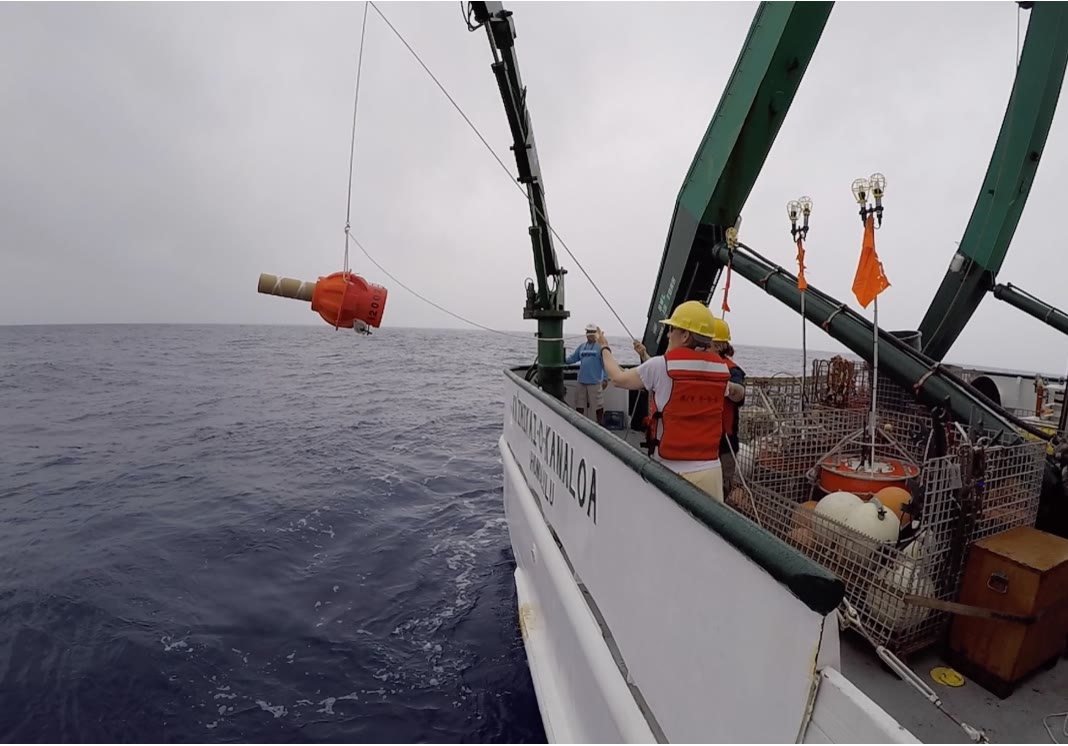
\includegraphics[width=0.6\linewidth]{images/book3/b1-deep-float.jpg}

{\small Een profilerende drijver voor de diepe oceaan (het oranje instrument dat aan de kraan hangt) wordt in 2018 van een onderzoeksschip neergelaten; eenmaal losgelaten zinkt hij tot zijn werkdiepte en komt hij met regelmatige tussenpozen aan het oppervlak om zijn gegevens te verzenden. (Onbekende fotograaf van NOAA, publiek domein, via Wikimedia Commons.)}
\label{fig:b1:ocean-circulation:float}
\end{omfigure}
% ledger: commons:deep-solo, noaa:argo-25

De omwenteling vervoert warmte. Water dat naar het noorden gaat warm en als koud water terugkomt, heeft zijn warmte aan de atmosfeer van het noorden afgegeven.

\begin{proposition}[Warmte vervoerd door een omwenteling]\label{prop:b1:ocean-circulation:heat}
Als een volumetransport $Q$ een \omterm{def:b1:spherical-astronomy:geographic}{breedtegraad} noordwaarts oversteekt bij de \omterm{def:b1:fluid-envelopes-structure:potential-temperature}{potentiële temperatuur}
$\theta_1$ en zuidwaarts terugkeert bij $\theta_2$, zonder netto transport van massa, voert de omwenteling de warmteflux noordwaarts:
\[
  H = \rho c_p\,Q\,(\theta_1 - \theta_2),
\]
waarin $c_p$ de specifieke warmte van zeewater is.
\end{proposition}
% ledger: teos10:cp0

\begin{proof}
Elke seconde steekt de massa $\rho Q$ noordwaarts over en draagt de warmte-inhoud $\rho Q
c_p\theta_1$, gerekend vanaf een willekeurig nulpunt van de temperatuur; dezelfde massa steekt zuidwaarts over met $\rho Q c_p\theta_2$. De netto noordwaartse flux is het verschil;
omdat de twee massa's gelijk zijn, valt het willekeurige nulpunt weg, en het resultaat is een echt warmtetransport.
\end{proof}

Een ruwe begroting van de Noord-Atlantische Oceaan, van W.~Schmitz, laat de Golfstroom \qty{40}{\sverdrup} water van \qty{18}{\celsius} naar het noorden voeren, waarvan
\qty{14}{\sverdrup} als diep water van \qty{2}{\celsius} naar het zuiden terugkeert. Met $c_p =
\qty{3992}{J.kg^{-1}.K^{-1}}$ en $\rho = \qty{1027}{kg.m^{-3}}$ voert deze omwenteling $1027 \times 3992 \times \num{14e6} \times 16 = \qty{0.92e15}{W}$, ongeveer
\qty{0.9}{PW}, noordelijk van \ang{24} N; zorgvuldige schattingen komen uit op \qty{1.2}{PW}, een kwart van het poolwaartse warmtetransport door atmosfeer en oceaan samen. Het grootste deel van deze warmte wordt aan de lucht boven het noordelijke deel van de Noord-Atlantische Oceaan afgegeven, wat een van de redenen is waarom Noorwegen, op \ang{60} N, veel warmer is dan het zuiden van Groenland op dezelfde \omterm{def:b1:spherical-astronomy:geographic}{breedtegraad}.
% ledger: stewart:heat-conveyor, rapid:home, teos10:cp0 (computed in calc/ch29.py)

De diepe circulatie is traag. Als het ongeveer duizend jaar kost voordat water dat in de Noord-Atlantische Oceaan zinkt via de Antarctische Circumpolaire Stroom de Noord-Pacifische Oceaan bereikt, is zijn gemiddelde snelheid ongeveer \qty{1}{mm/s}, honderd keer minder dan de wisselende diepe stromingen die een stroommeter registreert. Haar snelheid wordt daarom afgeleid uit tracers in plaats van gemeten: tritium, in de jaren vijftig door de kernproeven in de atmosfeer gebracht en met een halveringstijd van 12.3 jaar vervallend, drong het diepe Noord-Atlantische Oceaan binnen waar diep water vormt, en na 25 jaar had het zich nauwelijks ten zuiden van \ang{30} N verspreid, een gemiddelde snelheid van minder dan \qty{1}{mm/s}. Het volume van de oceaan gedeeld door de snelheid waarmee diep water vormt, geeft dezelfde orde van tijd (\cref{exo:b1:ocean-circulation:12}).
% ledger: stewart:deep-circulation, nos:conveyor

De Antarctische Circumpolaire Stroom verbindt de bekkens. Haar stromingen bereiken de zeebodem en zijn traag, ongeveer \qty{10}{cm/s}, tot \qty{50}{cm/s} aan haar fronten, maar zij is diep en breed: een reeks verankerde stroommeters over de Drakestraat, tussen Zuid-Amerika en Antarctica, gaf \qty[uncertainty-mode=separate]{125 \pm 11}{\sverdrup} (gepubliceerd in 1985), en een dichtere reeks in 2007--2011, die ook de stromingen nabij de bodem mat, gaf \qty{173.3}{\sverdrup}, \qty{39}{\percent} meer dan die lang gebruikte waarde. Zij voert diep water van elke oceaan naar de andere en mengt het onderweg.
% ledger: stewart:acc, donohue:acc

\begin{dated}{2021}
% ledger: ipcc:amoc-observed, ipcc:amoc-projected
Het IPCC-rapport uit 2021 stelt vast, uit reconstructies, dat de Atlantische omwenteling over de afgelopen \num{8000} jaar relatief stabiel was (\emph{gemiddeld vertrouwen}), met een verzwakking die in de late negentiende eeuw begon (\emph{gemiddeld vertrouwen}), maar heeft slechts \emph{laag vertrouwen} in een algemene afname gedurende de twintigste eeuw. De verzwakking die rechtstreeks is waargenomen van het midden van de jaren 2000 tot het midden van de jaren 2010 (\emph{hoog vertrouwen}) valt niet te onderscheiden van variabiliteit op de schaal van decennia (\emph{hoog vertrouwen}). De omwenteling zal \emph{zeer waarschijnlijk} in de eenentwintigste eeuw verzwakken voor alle emissiescenario's, met slechts \emph{laag vertrouwen} in de omvang van de afname; er is \emph{gemiddeld vertrouwen} dat zij vóór 2100 niet abrupt zal instorten.
\end{dated}

\section{Oefeningen}

\begin{exercise}[$\star$]\label{exo:b1:ocean-circulation:1}
Gebruik de bulkformule met $\rho_a = \qty{1.3}{kg.m^{-3}}$ en de weerstandscoëfficiënt
van Yelland en Taylor. (a)~Bereken $C_D$ en de \omterm{def:b1:ocean-circulation:wind-stress}{windschuifspanning} voor winden van 4, 7 en
\qty{15}{m/s}. (b)~Met welke factor groeit de spanning van 7 tot \qty{15}{m/s}?
Vergelijk dit met de verhouding van de kwadraten van de snelheden en verklaar het verschil.
% ledger: stewart:wind-stress, stewart:drag-coefficient
\end{exercise}

\begin{exercise}[$\star$]\label{exo:b1:ocean-circulation:2}
Geef de richting van het \omterm{def:b1:ocean-circulation:ekman}{Ekmantransport} in elk geval. (a)~Een wind die naar het oosten waait op \ang{45} N.
(b)~Een passaat uit het noordoosten op \ang{15} N. (c)~Een wind die naar het oosten waait op \ang{50} Z. (d)~Een wind uit het zuiden langs de
westkust van Zuid-Afrika, nabij \ang{23} Z. In welk van de vier gevallen wijst het transport naar zee, en wat volgt daaruit?
\end{exercise}

\begin{exercise}[$\star$]\label{exo:b1:ocean-circulation:3}
Op \ang{26.5} N in de Atlantische Oceaan zijn de gemiddelde transporten van 2004--2024: Straat van
Florida \qty{31.7}{\sverdrup}, Ekman \qty{3.5}{\sverdrup}, bovenste midoceaan
\qty{-17.9}{\sverdrup}; per laag: 0--\qty{800}{m} \qty{16.6}{\sverdrup},
800--\qty{1100}{m} \qty{0.4}{\sverdrup}, 1100--\qty{3000}{m} \qty{-12.0}{\sverdrup},
3000--\qty{5000}{m} \qty{-5.9}{\sverdrup} (noordwaarts positief). (a)~Tel de eerste drie op en vergelijk met de gepubliceerde omwenteling, \qty{17.1}{\sverdrup}. (b)~Vergelijk de noordwaartse stroming boven \qty{1100}{m} met de zuidwaartse stroming eronder. (c)~Reken \qty{17.1}{\sverdrup} om in kubieke kilometer per jaar, en bereken de tijd die deze stroming nodig zou hebben om het volume van de hele oceaan, \qty{1.3324e9}{km^3}, te vullen.
% ledger: rapid:transports, charette:ocean-volume
\end{exercise}

\begin{exercise}[$\star$]\label{exo:b1:ocean-circulation:4}
Bereken met de formules van Ekman de Ekmandiepte en de oppervlaktestroom bij een wind van
\qty{10}{m/s} op \ang{15}, \ang{45} en \ang{60} \omterm{def:b1:spherical-astronomy:geographic}{breedtegraad}, en de oppervlaktestroom als percentage van de wind. Waarom falen de formules nabij de evenaar?
% ledger: stewart:ekman-constants
\end{exercise}

\begin{exercise}[$\star\star$]\label{exo:b1:ocean-circulation:5}
Over \ang{11} N in de Atlantische Oceaan neem een gemiddelde \omterm{def:b1:ocean-circulation:wind-stress}{windschuifspanning} van \qty{0.07}{Pa} naar het
westen over een breedte van \qty{5000}{km}, en $\rho = \qty{1027}{kg.m^{-3}}$.
(a)~Bereken het \omterm{def:b1:ocean-circulation:ekman}{Ekmantransport} per meter en zijn richting. (b)~Bereken het totale volumetransport over de doorsnede in \omterm{def:b1:ocean-circulation:ekman}{sverdrups}. (c)~Vergelijk met de rechtstreeks gemeten
transporten ($12.0 \pm \qty{5.5}{\sverdrup}$) en met het transport berekend uit langjarige
winden ($13.5 \pm \qty{0.3}{\sverdrup}$).
% ledger: stewart:ekman-transport
\end{exercise}

\begin{exercise}[$\star\star$]\label{exo:b1:ocean-circulation:6}
Langs de equatoriale Stille Oceaan oefenen de \omterm{def:b1:atmospheric-circulation:winds}{passaten} een spanning van \qty{0.05}{Pa} uit
naar het westen. (a)~Bereken het \omterm{def:b1:ocean-circulation:ekman}{Ekmantransport} per meter, en zijn richting, op \ang{2} N en op \ang{2}~Z. (b)~Ervan uitgaande dat het water dat over deze twee breedtegraden wordt weggevoerd van onderaf tussen hen wordt vervangen, bereken de gemiddelde opwellingssnelheid in meter per dag. (c)~Wat gebeurt er met de formule van de stelling op de evenaar zelf? Welke conclusie blijft overeind?
\end{exercise}

\begin{exercise}[$\star\star$]\label{exo:b1:ocean-circulation:7}
Over een \omterm{def:b1:ocean-circulation:gyre}{subtropische gyre} neem een \omterm{def:b1:ocean-circulation:wind-stress}{windschuifspanning} van \qty{0.06}{Pa} naar het westen op
\ang{15} N en \qty{0.12}{Pa} naar het oosten op \ang{40} N. (a)~Bereken beide \omterm{def:b1:ocean-circulation:ekman}{Ekmantransporten} en hun richtingen. (b)~Ervan uitgaande dat het transport lineair verandert tussen de twee breedtegraden, bereken de verticale snelheid aan de basis van de \omterm{def:b1:ocean-circulation:ekman}{Ekmanlaag}, in meter per jaar, en zeg of zij omhoog of omlaag is. (c)~Hoeveel \omterm{def:b1:ocean-circulation:ekman}{sverdrups} worden over een bekken van \qty{5000}{km} breed door de basis van de laag gepompt?
\end{exercise}

\begin{exercise}[$\star\star$]\label{exo:b1:ocean-circulation:8}
Neem $\rho = \qty{1027}{kg.m^{-3}}$ en $c_p = \qty{3992}{J.kg^{-1}.K^{-1}}$.
(a)~Bereken de warmte die \qty{17}{\sverdrup} naar het noorden draagt, stromend naar het noorden bij
\qty{15}{\celsius} en terugkerend bij \qty{3}{\celsius}. (b)~Vergelijk met de \qty{1.2}{PW} die de Atlantische omwenteling draagt. (c)~Als hetzelfde water aan het oppervlak langs de oostzijde van het bekken, bij \qty{12}{\celsius}, zuidwaarts terugkeerde, welke warmte zou het dan dragen? Wat zegt dit over het belang van de \omterm{def:b1:ocean-circulation:moc}{vorming van diep water}?
% ledger: rapid:home, teos10:cp0
\end{exercise}

\begin{exercise}[$\star\star$]\label{exo:b1:ocean-circulation:9}
Drie \omterm{def:b1:fluid-envelopes-structure:ts-diagram}{watermassa}'s van de Zuidelijke Atlantische Oceaan hebben de potentiële temperaturen en zoutgehaltes: Antarctisch Tussenwater \qty{3.3}{\celsius}, 34.15; Noord-Atlantisch Diepwater \qty{4.0}{\celsius}, 35.00; Antarctisch Bodemwater \qty{0.4}{\celsius},
34.67. Een monster op diepte heeft $\theta = \qty{2.78}{\celsius}$ en $S = 34.731$.
Gebruik \cref{prop:b1:fluid-envelopes-structure:mixing} om het aandeel van elke \omterm{def:b1:fluid-envelopes-structure:ts-diagram}{watermassa} in het monster te bepalen.
% ledger: stewart:deep-circulation
\end{exercise}

\begin{exercise}[$\star\star\star$]\label{exo:b1:ocean-circulation:10}
Neem de spiraal van \cref{prop:b1:ocean-circulation:spiral}. (a)~Toon aan dat $u$ en $v$ voldoen aan $f v + A_z u'' = 0$ en $-f u + A_z v'' = 0$. (Hint: schrijf $u + iv =
V_0\,e^{i\pi/4}\,e^{(1+i)az}$.) (b)~Toon aan dat de spanning $\rho A_z\,\partial\vec
v/\partial z$ aan het oppervlak gelijk is aan de \omterm{def:b1:ocean-circulation:wind-stress}{windschuifspanning} $(0, T)$. (c)~Bereken de
transporten $\int_{-\infty}^0 \rho u\,\mathrm dz$ en $\int_{-\infty}^0 \rho
v\,\mathrm dz$, en controleer of zij overeenkomen met
\cref{thm:b1:ocean-circulation:ekman}.
\end{exercise}

\begin{exercise}[$\star\star\star$]\label{exo:b1:ocean-circulation:11}
In Stommels model heeft de \omterm{def:b1:ocean-circulation:wbc}{westelijke randstroom} een breedte van ongeveer $R/\beta$,
waar $R$ de snelheid van de bodemwrijving is en $\beta = \mathrm df/\mathrm dy$ de noordwaartse toename van de \omterm{def:b1:atmospheric-circulation:coriolis-parameter}{Coriolisparameter}. (a)~Toon aan dat $\beta = 2\Omega
\cos\varphi/a_\oplus$ en bereken hem op \ang{30} N ($a_\oplus = \qty{6371}{km}$). (b)~Met $R = \qty{e-6}{s^{-1}}$ bereken de breedte. (c)~Een transport van
\qty{30}{\sverdrup} stroomt zuidwaarts over het inwendige van een bekken van \qty{5000}{km} breed
in de bovenste \qty{1000}{m}, en keert noordwaarts terug in de randstroom over dezelfde diepte. Bereken beide gemiddelde snelheden en vergelijk ze met de snelheid van de Golfstroom, \qty{1.8}{m/s}.
% ledger: stewart:north-atlantic, nos:gulf-stream, earth:Rmean
\end{exercise}

\begin{exercise}[$\star\star\star$]\label{exo:b1:ocean-circulation:12}
De oceaan bevat \qty{1.3324e9}{km^3} over \qty{361.84e6}{km^2}. (a)~Toon aan dat het volume onder \qty{1000}{m} ten minste \qty{9.71e8}{km^3} is. (b)~Noord-Atlantisch Diepwater vormt aan ongeveer \qty{17}{\sverdrup} en Antarctisch Bodemwater aan ongeveer
\qty{9}{\sverdrup}. Schat de tijd die nodig is om het water onder \qty{1000}{m} te vernieuwen, en vergelijk die met de duizend jaar van het transportband. (c)~Tritium heeft een halveringstijd van 12.3 jaar. Welk deel van een tritiuminvoer blijft over na 25 jaar? Hoe ver reist water dat zich met \qty{1}{mm/s} beweegt in 25 jaar?
% ledger: charette:ocean-volume, stewart:deep-circulation, stewart:acc, rapid:transports
\end{exercise}

\section{Probleem: een opwellingskust}

\begin{problem}[{Weekendprobleem --- een zomerwind langs een kust op \ang{38} N}]
\label{pb:b1:ocean-circulation:1}
% values: calc/ch29.py (invented coast; constants from the ledger)
Een rechte kust loopt noord--zuid op \ang{38} N, met de oceaan naar het westen. In de zomer waait er weken lang een gestage wind van \qty{8}{m/s} uit het noorden langs haar. De kust is verzonnen, maar haar getallen zijn typisch voor de oostzijden van de oceanen.
Gebruik $\Omega = 2\pi/(\qty{23.9345}{h})$, $\rho_a = \qty{1.3}{kg.m^{-3}}$, de weerstandscoëfficiënt van Yelland en Taylor, $\rho = \qty{1027}{kg.m^{-3}}$ voor zeewater en
$c_p = \qty{3992}{J.kg^{-1}.K^{-1}}$.

\medskip
\noindent\textbf{Deel I --- De wind en zijn spanning.}
\begin{enumerate}
  \item Naar welke richting waait de wind? Is hij langs de kust of er dwars op?
  \item Bereken de weerstandscoëfficiënt.
  \item Bereken de \omterm{def:b1:ocean-circulation:wind-stress}{windschuifspanning}.
  \item Dezelfde twee vragen voor een wind van \qty{12}{m/s}. Met welke factor groeit de spanning, en waarom is zij meer dan de verhouding van de kwadraten van de snelheden?
  \item Bereken de \omterm{def:b1:atmospheric-circulation:coriolis-parameter}{Coriolisparameter} op \ang{38} N.
  \item Bereken $2\pi/f$ in uren. Waarom moet de wind een dag of langer waaien voordat het Ekmanevenwicht van toepassing is?
\end{enumerate}

\medskip
\noindent\textbf{Deel II --- De Ekmanlaag.}
\begin{enumerate}[resume]
  \item In welke richting gaat het \omterm{def:b1:ocean-circulation:ekman}{Ekmantransport}? Naar het land of naar de open zee?
  \item Bereken het Ekman-massatransport per meter kust.
  \item Reken het om in een volumetransport per meter.
  \item Bereken de Ekmandiepte met de formule van Ekman.
  \item Bereken de gemiddelde snelheid naar zee in de laag, in \unit{cm/s}.
  \item Bereken de oppervlaktestroom met de formule van Ekman, en haar richting. Wat suggereren de metingen van drijvers in plaats daarvan voor haar snelheid?
\end{enumerate}

\medskip
\noindent\textbf{Deel III --- Opwelling aan de kust.}
\begin{enumerate}[resume]
  \item Verklaar, met een schets van een verticale doorsnede, waar het water vandaan komt dat naar zee wordt meegevoerd.
  \item Bereken het volume dat per dag langs elke kilometer kust opwelt.
  \item Stel dat het water omhoog stroomt door een band van \qty{20}{km} breed langs de kust. Bereken de gemiddelde opwaartse snelheid, in \unit{m/s} en in meter per dag.
  \item Hoe lang doet het water over van de basis van de \omterm{def:b1:ocean-circulation:ekman}{Ekmanlaag} tot het oppervlak bij deze snelheid?
  \item Het opgewelde water bereikt het oppervlak bij \qty{12}{\celsius}, terwijl de open zee voor de kust \qty{18}{\celsius} is. De zeewind voert warme, vochtige lucht van zee over dit water. Wat gebeurt er met de lucht nabij het oppervlak, en welk weer volgt aan de kust?
  \item Waarom zijn zulke kusten rijk aan vis?
  \item In de herfst draait de wind en waait hij een week lang uit het zuiden. Wat gebeurt er met het transport en met het water aan de kust?
\end{enumerate}

\medskip
\noindent\textbf{Deel IV --- Andere kusten en het totale transport.}
\begin{enumerate}[resume]
  \item Bereken met dezelfde spanning het \omterm{def:b1:ocean-circulation:ekman}{Ekmantransport} per meter op \ang{20} N en vergelijk het met \ang{38} N.
  \item Welke windrichting drijft \omterm{def:b1:ocean-circulation:upwelling}{opwelling} aan op de westkust van Zuid-Afrika, nabij \ang{23} Z? Vergelijk met de kust van het vraagstuk.
  \item Bereken bij een wind van \qty{5}{m/s} in plaats van \qty{8}{m/s} op \ang{38} N de spanning en het \omterm{def:b1:ocean-circulation:ekman}{Ekmantransport} per meter, en hun verhouding tot die van vraag~8.
  \item Het opgewelde water warmt met \qty{6}{\celsius} op terwijl het naar zee drijft. Bereken de warmte die het per seconde per meter kust opneemt, en dan over \qty{1000}{km}.
  \item Hoe lang moet een kust van zulk type zijn om even veel water op te wellen als de Golfstroom door de Straat van Florida voert, \qty{31.7}{\sverdrup}?
  \item Welk volume water, in \omterm{def:b1:ocean-circulation:ekman}{sverdrups}, wordt langs \qty{1000}{km} van deze kust opgewelt?
\end{enumerate}
\end{problem}
